\documentclass[12pt]{article}

\usepackage{lmodern}
\usepackage[T1]{fontenc}
\usepackage{amsmath}
\usepackage{amsthm}
\usepackage{amssymb}
\usepackage{url}
\usepackage{latexsym}
%\usepackage{titlefoot}
\usepackage[small]{titlesec}
\usepackage[small,it]{caption}
\usepackage{mathtools} % for mathclap

%document specific packages
\usepackage[table]{xcolor}
\usepackage[margin=0.75in]{geometry}
\usepackage{mathrsfs}
\usepackage{tikz}
\usepackage{tkz-graph}
\usepackage{tkz-berge}
\usetikzlibrary{decorations.pathreplacing,decorations.markings}
\usetikzlibrary{cd}
\usepackage{diagbox}
\usepackage{pdflscape}
\usetikzlibrary{shapes.misc}

\newcommand{\Z}{\mathbb{Z}}
\newcommand{\Q}{\mathbb{Q}}
\newcommand{\R}{\mathbb{R}}
\newcommand{\C}{\mathbb{C}}
\newcommand{\N}{\mathbb{N}}
\newcommand{\F}{\mathbb{F}}
\newcommand{\CP}{\mathbb{CP}}
\newcommand{\Sphere}{\mathbb{S}}
\newcommand{\defas}{:=}
\newcommand{\floor}[1]{\lfloor {#1} \rfloor}
\newcommand{\ceil}[1]{\lceil {#1} \rceil}
\newcommand{\abs}[1]{\lvert {#1} \rvert}
\newcommand{\bracket}[1]{\left[ {#1} \right]}
\newcommand{\para}[1]{\left( {#1} \right)}
\newcommand{\brac}[1]{\left\{ {#1} \right\}}
\newcommand{\innerprod}[2]{\langle {#1},{#2} \rangle}
\newcommand{\sumover}[3]{\sum_{{#1}}^{{#2}}{{#3}}}
\newcommand{\prodover}[3]{\prod_{{#1}}^{{#2}}{{#3}}}
\newcommand{\intover}[4]{\int_{{#1}}^{{#2}}{{#3} \mathrm{d}{#4}}}
\newcommand{\norm}[1]{\left\| {#1} \right\|}
\newcommand{\seq}[2]{({#1})_{{#2} = 1}^{\infty}}
\newcommand{\limit}[3]{\lim_{#1 \to #2}{#3}}
\newcommand{\Image}{\operatorname{Im}}
\newcommand{\Ker}{\text{Ker}}
\newcommand{\angleb}[1]{\langle {#1} \rangle}
\newcommand{\quotemarks}[1]{``{#1}''}
\newcommand{\Aff}{\operatorname{Aff}}
\newcommand{\Id}{\operatorname{Id}}
\newcommand{\GL}{\operatorname{GL}}
\newcommand{\SL}{\operatorname{SL}}
\newcommand{\Sp}{\operatorname{Sp}}
%\newcommand{\SO}{\operatorname{SO}}
\newcommand{\Hom}{\operatorname{Hom}}
\newcommand{\Det}{\operatorname{Det}}
\newcommand{\Dim}{\operatorname{Dim}}
\newcommand{\Trace}{\operatorname{Trace}}
\newcommand{\wt}[1]{\widetilde{{#1}}}
\newcommand{\transpose}[1]{{}^t{#1}}
\newcommand{\restricto}[2]{\left.{#1}\right|_{{#2}}}
\newcommand{\ignore}[1]{}

%%%%%%%%%%%%%%%%% 
%macros for chord diagrams
%%%%%%%%%%%%%%%%%
\usetikzlibrary{decorations.pathmorphing,calc}
\usetikzlibrary{intersections}                                                   

\tikzstyle{propagator}=[decorate,decoration={snake,amplitude=0.8mm}]

\newcommand{\drawboundary}[2]{
	\pgfmathsetmacro{\n}{#1}
	\pgfmathsetmacro{\radius}{#2}
	\pgfmathsetmacro{\angle}{360/\n}
	\draw (0,0) circle (\radius);
	\foreach \i in {1,2,...,\n} {
		\draw (\angle*\i+ \angle/2:\radius) node {$\bullet$};
	}	
}


\newcommand{\drawchord}[3]{
	\pgfmathsetmacro{\r}{#1}
	\pgfmathsetmacro{\s}{#2}
	
	\begin{scope}
		\draw[#3] (\angle*\r + \angle/2:\radius) -- (\angle*\s + \angle/2:\radius);
	\end{scope}
}


\newcommand{\drawnumbers}{
	\foreach \i in {1,2,...,\n} {
		\pgfmathsetmacro{\x}{\angle*\i}
		\draw (\x:\radius*1.15) node {\footnotesize \i};
	}
}

\newcommand{\drawnumbersshift}{
	\foreach \i in {1,2,...,\n} {
		\pgfmathsetmacro{\x}{\angle*\i + \angle/2}
		\draw (\x:\radius*1.15) node {\footnotesize \i};
	}
}



 
\begin{document}

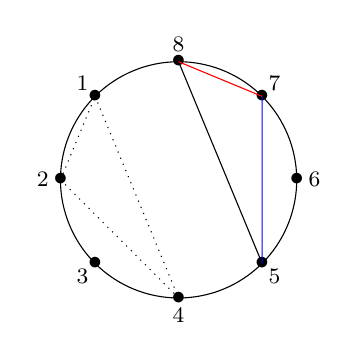
\begin{tikzpicture}[rotate=67.5,baseline=(current bounding box.east)]
	\begin{scope}
		\drawboundary{8}{1.5}
		\drawnumbersshift
		\drawchord{1}{4}{dotted}
		\drawchord{2}{4}{dotted}
		\drawchord{2}{1}{dotted}
		\drawchord{5}{8}{}
		\drawchord{5}{7}{blue}
		\drawchord{7}{8}{red}
		
	\end{scope}
\end{tikzpicture} 


	\begin{center}
		\scalebox{1}{
			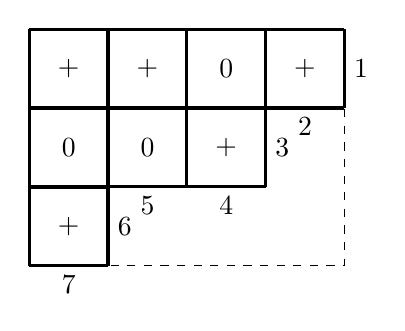
\begin{tikzpicture}[scale=1]
				\draw[dashed] (0,0) rectangle (4,3);
				\draw[very thick] (0,0) grid ++(1,1);
				\draw[very thick] (0,1) grid ++(3,1);
				\draw[very thick] (0,2) grid ++(4,1);
				
				\node at (0.5,0.5) {+};
				\node at (0.5,1.5) {0};
				\node at (1.5,1.5) {0};
				\node at (2.5,1.5) {+};
				\node at (0.5,2.5) {+};
				\node at (1.5,2.5) {+};
				\node at (2.5,2.5) {0};
				\node at (3.5,2.5) {+};
				
				\node[right] at (4  ,2.5) {1};
				\node[below] at (3.5,2  ) {2};
				\node[right] at (3  ,1.5) {3};
				\node[below] at (2.5,1  ) {4};
				\node[below] at (1.5,1  ) {5};
				\node[right] at (1  ,0.5) {6};
				\node[below] at (0.5,0  ) {7};
			\end{tikzpicture}

	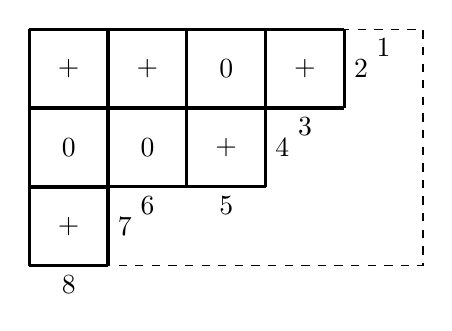
\begin{tikzpicture}[scale=1]
		\draw[dashed] (0,0) rectangle (5,3);
		\draw[very thick] (0,0) grid ++(1,1);
		\draw[very thick] (0,1) grid ++(3,1);
		\draw[very thick] (0,2) grid ++(4,1);
		
		\node at (0.5,0.5) {+};
		\node at (0.5,1.5) {0};
		\node at (1.5,1.5) {0};
		\node at (2.5,1.5) {+};
		\node at (0.5,2.5) {+};
		\node at (1.5,2.5) {+};
		\node at (2.5,2.5) {0};
		\node at (3.5,2.5) {+};
		
		\node[below] at ( 4.5 ,3) {1};
		\node[right] at (4  ,2.5) {2};
		\node[below] at (3.5,2  ) {3};
		\node[right] at (3  ,1.5) {4};
		\node[below] at (2.5,1  ) {5};
		\node[below] at (1.5,1  ) {6};
		\node[right] at (1  ,0.5) {7};
		\node[below] at (0.5,0  ) {8};
	\end{tikzpicture}
}


	
		\scalebox{1}{
			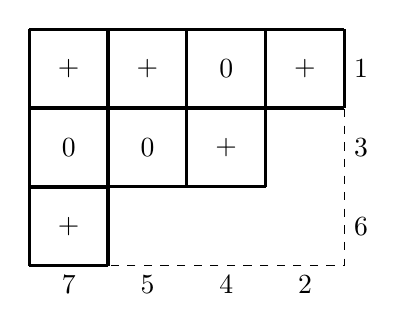
\begin{tikzpicture}[scale=1]
				\draw[dashed] (0,0) rectangle (4,3);
				\draw[very thick] (0,0) grid ++(1,1);
				\draw[very thick] (0,1) grid ++(3,1);
				\draw[very thick] (0,2) grid ++(4,1);
				
				\node at (0.5,0.5) {+};
				\node at (0.5,1.5) {0};
				\node at (1.5,1.5) {0};
				\node at (2.5,1.5) {+};
				\node at (0.5,2.5) {+};
				\node at (1.5,2.5) {+};
				\node at (2.5,2.5) {0};
				\node at (3.5,2.5) {+};
				
				\node[right] at (4  ,2.5) {1};
				\node[below] at (3.5,0  ) {2};
				\node[right] at (4  ,1.5) {3};
				\node[below] at (2.5,0  ) {4};
				\node[below] at (1.5,0  ) {5};
				\node[right] at (4  ,0.5) {6};
				\node[below] at (0.5,0  ) {7};
			\end{tikzpicture}
		}
		\scalebox{1}{
			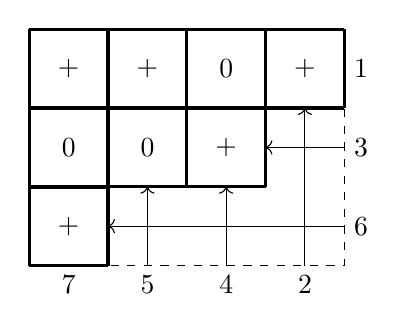
\begin{tikzpicture}[scale=1]
				\draw[dashed] (0,0) rectangle (4,3);
				\draw[very thick] (0,0) grid ++(1,1);
				\draw[very thick] (0,1) grid ++(3,1);
				\draw[very thick] (0,2) grid ++(4,1);
				
				\node at (0.5,0.5) {+};
				\node at (0.5,1.5) {0};
				\node at (1.5,1.5) {0};
				\node at (2.5,1.5) {+};
				\node at (0.5,2.5) {+};
				\node at (1.5,2.5) {+};
				\node at (2.5,2.5) {0};
				\node at (3.5,2.5) {+};
				
				\node[right] at (4  ,2.5) {1};
				\node[below] at (3.5,0  ) {2};
				\node[right] at (4  ,1.5) {3};
				\node[below] at (2.5,0  ) {4};
				\node[below] at (1.5,0  ) {5};
				\node[right] at (4  ,0.5) {6};
				\node[below] at (0.5,0  ) {7};
				
				\draw[->] (1.5,0) -- (1.5,1);
				\draw[->] (2.5,0) -- (2.5,1);
				\draw[->] (3.5,0) -- (3.5,2);
				\draw[->] (4,1.5) -- (3,1.5);
				\draw[->] (4,0.5) -- (1,0.5);
			\end{tikzpicture}
		}
		
		\scalebox{1}{
			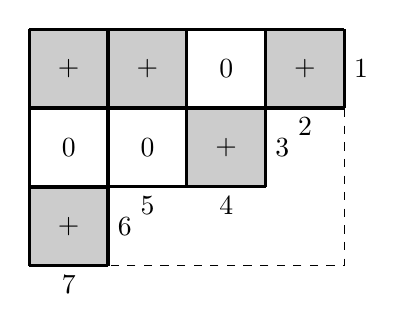
\begin{tikzpicture}[scale=1]
			
				\draw[fill=white!80!black] (0,0) rectangle ++(1,1);
				\draw[fill=white!80!black] (2,1) rectangle ++(1,1);
				\draw[fill=white!80!black] (0,2) rectangle ++(1,1);
				\draw[fill=white!80!black] (1,2) rectangle ++(1,1);
				\draw[fill=white!80!black] (3,2) rectangle ++(1,1);
				
				\draw[dashed] (0,0) rectangle (4,3);
				\draw[very thick] (0,0) grid ++(1,1);
				\draw[very thick] (0,1) grid ++(3,1);
				\draw[very thick] (0,2) grid ++(4,1);
				
				\node at (0.5,0.5) {+};
				\node at (0.5,1.5) {0};
				\node at (1.5,1.5) {0};
				\node at (2.5,1.5) {+};
				\node at (0.5,2.5) {+};
				\node at (1.5,2.5) {+};
				\node at (2.5,2.5) {0};
				\node at (3.5,2.5) {+};
				
				\node[right] at (4  ,2.5) {1};
				\node[below] at (3.5,2  ) {2};
				\node[right] at (3  ,1.5) {3};
				\node[below] at (2.5,1  ) {4};
				\node[below] at (1.5,1  ) {5};
				\node[right] at (1  ,0.5) {6};
				\node[below] at (0.5,0  ) {7};
			\end{tikzpicture}
		}
		\scalebox{1}{
			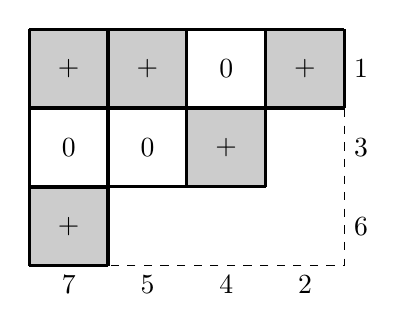
\begin{tikzpicture}[scale=1]
			
				\draw[fill=white!80!black] (0,0) rectangle ++(1,1);
				\draw[fill=white!80!black] (2,1) rectangle ++(1,1);
				\draw[fill=white!80!black] (0,2) rectangle ++(1,1);
				\draw[fill=white!80!black] (1,2) rectangle ++(1,1);
				\draw[fill=white!80!black] (3,2) rectangle ++(1,1);
				
				\draw[dashed] (0,0) rectangle (4,3);
				\draw[very thick] (0,0) grid ++(1,1);
				\draw[very thick] (0,1) grid ++(3,1);
				\draw[very thick] (0,2) grid ++(4,1);
				
				\node at (0.5,0.5) {+};
				\node at (0.5,1.5) {0};
				\node at (1.5,1.5) {0};
				\node at (2.5,1.5) {+};
				\node at (0.5,2.5) {+};
				\node at (1.5,2.5) {+};
				\node at (2.5,2.5) {0};
				\node at (3.5,2.5) {+};
				
				\node[right] at (4  ,2.5) {1};
				\node[below] at (3.5,0  ) {2};
				\node[right] at (4  ,1.5) {3};
				\node[below] at (2.5,0  ) {4};
				\node[below] at (1.5,0  ) {5};
				\node[right] at (4  ,0.5) {6};
				\node[below] at (0.5,0  ) {7};
			\end{tikzpicture}
		}
		\scalebox{1}{
			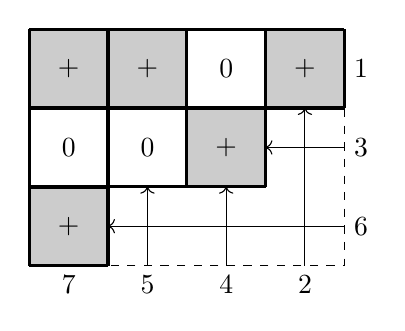
\begin{tikzpicture}[scale=1]
			
				\draw[fill=white!80!black] (0,0) rectangle ++(1,1);
				\draw[fill=white!80!black] (2,1) rectangle ++(1,1);
				\draw[fill=white!80!black] (0,2) rectangle ++(1,1);
				\draw[fill=white!80!black] (1,2) rectangle ++(1,1);
				\draw[fill=white!80!black] (3,2) rectangle ++(1,1);
				
				\draw[dashed] (0,0) rectangle (4,3);
				\draw[very thick] (0,0) grid ++(1,1);
				\draw[very thick] (0,1) grid ++(3,1);
				\draw[very thick] (0,2) grid ++(4,1);
				
				\node at (0.5,0.5) {+};
				\node at (0.5,1.5) {0};
				\node at (1.5,1.5) {0};
				\node at (2.5,1.5) {+};
				\node at (0.5,2.5) {+};
				\node at (1.5,2.5) {+};
				\node at (2.5,2.5) {0};
				\node at (3.5,2.5) {+};
				
				\draw[->] (1.5,0) -- (1.5,1);
				\draw[->] (2.5,0) -- (2.5,1);
				\draw[->] (3.5,0) -- (3.5,2);
				\draw[->] (4,1.5) -- (3,1.5);
				\draw[->] (4,0.5) -- (1,0.5);
				
				\node[right] at (4  ,2.5) {1};
				\node[below] at (3.5,0  ) {2};
				\node[right] at (4  ,1.5) {3};
				\node[below] at (2.5,0  ) {4};
				\node[below] at (1.5,0  ) {5};
				\node[right] at (4  ,0.5) {6};
				\node[below] at (0.5,0  ) {7};
			\end{tikzpicture}
		}
		
		\scalebox{1}{
			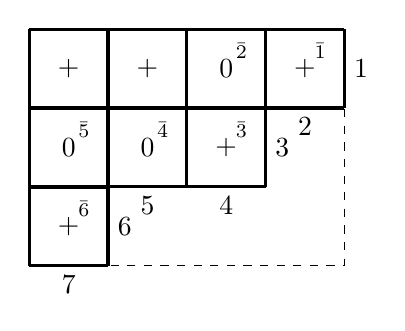
\begin{tikzpicture}[scale=1]			
				\draw[dashed] (0,0) rectangle (4,3);
				\draw[very thick] (0,0) grid ++(1,1);
				\draw[very thick] (0,1) grid ++(3,1);
				\draw[very thick] (0,2) grid ++(4,1);
				
				\node at (0.5,0.5) {+};
				\node at (0.5,1.5) {0};
				\node at (1.5,1.5) {0};
				\node at (2.5,1.5) {+};
				\node at (0.5,2.5) {+};
				\node at (1.5,2.5) {+};
				\node at (2.5,2.5) {0};
				\node at (3.5,2.5) {+};
				
				\node[right] at (4  ,2.5) {1};
				\node[below] at (3.5,2  ) {2};
				\node[right] at (3  ,1.5) {3};
				\node[below] at (2.5,1  ) {4};
				\node[below] at (1.5,1  ) {5};
				\node[right] at (1  ,0.5) {6};
				\node[below] at (0.5,0  ) {7};
				
				\node[above right] at (3.5  ,2.5) {$\scriptstyle\bar{1}$};
				\node[above right] at (2.5  ,2.5) {$\scriptstyle\bar{2}$};
				\node[above right] at (2.5  ,1.5) {$\scriptstyle\bar{3}$};
				\node[above right] at (1.5  ,1.5) {$\scriptstyle\bar{4}$};
				\node[above right] at (0.5  ,1.5) {$\scriptstyle\bar{5}$};
				\node[above right] at (0.5  ,0.5) {$\scriptstyle\bar{6}$};
			\end{tikzpicture}
		}	
		\scalebox{1}{
			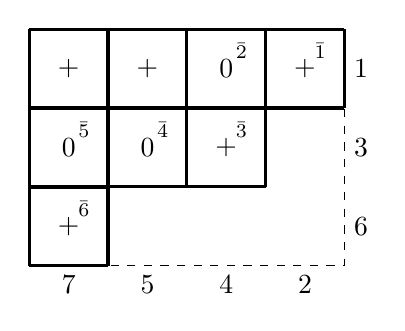
\begin{tikzpicture}[scale=1]			
				\draw[dashed] (0,0) rectangle (4,3);
				\draw[very thick] (0,0) grid ++(1,1);
				\draw[very thick] (0,1) grid ++(3,1);
				\draw[very thick] (0,2) grid ++(4,1);
				
				\node at (0.5,0.5) {+};
				\node at (0.5,1.5) {0};
				\node at (1.5,1.5) {0};
				\node at (2.5,1.5) {+};
				\node at (0.5,2.5) {+};
				\node at (1.5,2.5) {+};
				\node at (2.5,2.5) {0};
				\node at (3.5,2.5) {+};
				
				\node[right] at (4  ,2.5) {1};
				\node[below] at (3.5,0  ) {2};
				\node[right] at (4  ,1.5) {3};
				\node[below] at (2.5,0  ) {4};
				\node[below] at (1.5,0  ) {5};
				\node[right] at (4  ,0.5) {6};
				\node[below] at (0.5,0  ) {7};
				
				\node[above right] at (3.5  ,2.5) {$\scriptstyle\bar{1}$};
				\node[above right] at (2.5  ,2.5) {$\scriptstyle\bar{2}$};
				\node[above right] at (2.5  ,1.5) {$\scriptstyle\bar{3}$};
				\node[above right] at (1.5  ,1.5) {$\scriptstyle\bar{4}$};
				\node[above right] at (0.5  ,1.5) {$\scriptstyle\bar{5}$};
				\node[above right] at (0.5  ,0.5) {$\scriptstyle\bar{6}$};
			\end{tikzpicture}
		}
		\scalebox{1}{
			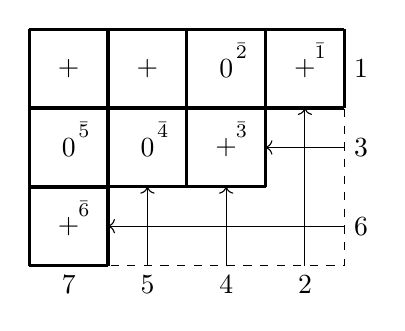
\begin{tikzpicture}[scale=1]			
				\draw[dashed] (0,0) rectangle (4,3);
				\draw[very thick] (0,0) grid ++(1,1);
				\draw[very thick] (0,1) grid ++(3,1);
				\draw[very thick] (0,2) grid ++(4,1);
				
				\node at (0.5,0.5) {+};
				\node at (0.5,1.5) {0};
				\node at (1.5,1.5) {0};
				\node at (2.5,1.5) {+};
				\node at (0.5,2.5) {+};
				\node at (1.5,2.5) {+};
				\node at (2.5,2.5) {0};
				\node at (3.5,2.5) {+};
				
				\node[right] at (4  ,2.5) {1};
				\node[below] at (3.5,0  ) {2};
				\node[right] at (4  ,1.5) {3};
				\node[below] at (2.5,0  ) {4};
				\node[below] at (1.5,0  ) {5};
				\node[right] at (4  ,0.5) {6};
				\node[below] at (0.5,0  ) {7};
				
				\draw[->] (1.5,0) -- (1.5,1);
				\draw[->] (2.5,0) -- (2.5,1);
				\draw[->] (3.5,0) -- (3.5,2);
				\draw[->] (4,1.5) -- (3,1.5);
				\draw[->] (4,0.5) -- (1,0.5);
				
				\node[above right] at (3.5  ,2.5) {$\scriptstyle\bar{1}$};
				\node[above right] at (2.5  ,2.5) {$\scriptstyle\bar{2}$};
				\node[above right] at (2.5  ,1.5) {$\scriptstyle\bar{3}$};
				\node[above right] at (1.5  ,1.5) {$\scriptstyle\bar{4}$};
				\node[above right] at (0.5  ,1.5) {$\scriptstyle\bar{5}$};
				\node[above right] at (0.5  ,0.5) {$\scriptstyle\bar{6}$};
			\end{tikzpicture}
		}
		
		\scalebox{1}{
		
			\tikzset{cross/.style={cross out, draw=black, minimum size=2*(#1-\pgflinewidth), inner sep=0pt, outer sep=0pt},
			%default radius will be 1pt. 
			cross/.default={10pt}}

			\begin{tikzpicture}[scale=1]			
				\draw[dashed] (0,0) rectangle (4,3);
				\draw[very thick] (0,0) grid ++(1,1);
				\draw[very thick] (0,1) grid ++(3,1);
				\draw[very thick] (0,2) grid ++(4,1);
				
				\node at (0.5,0.5) {+};
				\node at (0.5,1.5) {0};
				\node at (1.5,1.5) {0};
				\node[draw,circle] at (2.5,1.5) {+};
				\node at (0.5,2.5) {+};
				\node[draw,circle] at (1.5,2.5) {+};
				\node at (2.5,2.5) {0};
				\node at (3.5,2.5) {+};
				
				\node[cross,right] at (4  ,2.5) {1};
				\node[cross,below] at (3.5,0  ) {2};
				\node[cross,right] at (4  ,1.5) {3};
				\node[draw,circle,below] at (2.5,0  ) {4};
				\node[draw,circle,below] at (1.5,0  ) {5};
				\node[draw,circle,right] at (4  ,0.5) {6};
				\node[cross,below] at (0.5,0  ) {7};
				
				\node[above right] at (3.5  ,2.5) {$\scriptstyle\bar{1}$};
				\node[above right] at (2.5  ,2.5) {$\scriptstyle\bar{2}$};
				\node[above right] at (2.5  ,1.5) {$\scriptstyle\bar{3}$};
				\node[above right] at (1.5  ,1.5) {$\scriptstyle\bar{4}$};
				\node[above right] at (0.5  ,1.5) {$\scriptstyle\bar{5}$};
				\node[above right] at (0.5  ,0.5) {$\scriptstyle\bar{6}$};
			\end{tikzpicture}
		}
	\end{center}

\end{document}




